\chapter{相关理论基础与关键技术} \section{时间序列预测基础} 时间序列数据是按照时间顺序采集的一组观测值，通常可以表示为按时间排列的单变量序列或多变量向量序列，其中 $t$ 表示时间步，$T$ 为序列长度。对于单变量时间序列，每个时刻只有一个标量观测；对于多元时间序列，每个时刻包含多个通道（变量）的联合观测。时间序列通常同时包含长期趋势、季节性（周期性）、局部波动以及随机噪声等成分，这些成分在时间轴上叠加并相互作用，使得对其进行建模与预测具有较高难度。通过从历史观测中挖掘这些潜在模式，可以为需求规划、资源调度、风险预警和策略制定提供关键支持。 一般地，时间序列预测（Time Series Forecasting, TSF）的目标是利用历史观测值估计未来一段时间内的序列取值，可形式化为从过去窗口到未来窗口的映射。对于单变量时间序列预测问题，给定长度为 $p$ 的历史窗口，预测模型根据过去观测估计未来 $h$ 个时间步的取值。当预测步长为 1 时属于单步预测，更关注一步前的短期变化；当预测步长大于 1 时属于多步预测，需要同时考虑误差在时间上的累积效应。 在多元时间序列预测（Multivariate Time Series Forecasting, MTSF）中，模型同时利用多个相关变量的历史信息。若将过去 $p+1$ 个时间步组成一个多元观测窗口、未来 $h$ 个时间步组成预测窗口，则有 \begin{equation} \hat{\mathbf{X}}_{t+1:t+h} = f_\theta\bigl(\mathbf{X}_{t-p:t}\bigr)
\label{eq:chap2-02}
\end{equation}
与单变量情形相比，多元建模可以显式利用不同通道之间的相关性与协同关系，在能源、交通、金融等场景中往往能够获得更高的预测精度，但同时也带来了更高的维度、建模复杂度以及过拟合风险。 从预测时间跨度的角度，时间序列预测可粗略分为短期时间序列预测（Short-Term Time Series Forecasting, STSF）和长期时间序列预测（Long-Term Time Series Forecasting, LTSF）。前者通常对应较小的预测步长，用于实时控制、库存管理等需要快速响应的场景，对近期局部模式的建模能力要求更高；后者则对应较大的预测步长，往往需要模型在较长时间范围内同时把握长期趋势与多尺度周期结构，对模型的表达能力、误差累积控制以及泛化性能提出更高要求。相关中文综述也从时空序列预测与深度学习建模两个视角梳理了该领域的发展脉络，也说明多变量关联建模与复杂场景预测已成为时间序列研究的重要方向\cite{liu2021spatiotemporalcn}。本文聚焦的多元长程时间序列预测任务，即是在上述 MTSF 框架下、针对较大预测步长的情形，对模型在复杂动态与长程依赖条件下的建模能力进行系统研究。 \subsection{时间序列预测问题定义} 形式上，时间序列预测可以视为从过去观测窗口到未来预测窗口的映射学习问题。设给定的数据集由 $N$ 条多元时间序列样本组成，第 $n$ 个样本的序列长度记为 $T_n$，每个时间步都包含多个变量。在给定预测步长 $h$ 和历史窗口长度 $p$ 的情况下，多元长程时间序列预测任务可定义为：对任意满足条件的时间索引 $t$，利用长度为 $p+1$ 的历史窗口预测未来 $h$ 个时间步的序列。训练阶段的目标是利用训练集最小化某一损失函数（如 MSE 或 MAE）在所有样本与时间位置上的经验风险，即 \begin{equation}
\min_{\theta} \; \mathcal{L}(\theta) = \frac{1}{|\mathcal{S}|} \sum_{(n,t)\in \mathcal{S}} \ell\!\left(\hat{\mathbf{X}}^{(n)}_{t+1:t+h}, \mathbf{X}^{(n)}_{t+1:t+h}\right)
\label{eq:chap2-06}
\end{equation}
其中，$\mathcal{S}$ 表示所有可用的样本-时间对索引集合，$\ell(\cdot,\cdot)$ 表示逐样本损失函数。推理阶段，在给定新的历史窗口后，模型根据学习得到的参数输出对应的未来预测。在后续小节中，本文将围绕 MSE 与 MAE 两种常用评价指标的数学特性与适用场景，对上述损失函数进行更为细致的讨论。
\subsection{评价指标}
在时间序列预测任务中，均方误差（Mean Squared Error, MSE）和平均绝对误差（Mean Absolute Error, MAE）是最常用的两类评价指标，它们从不同角度刻画预测值与真实值之间的偏差，对模型训练目标与应用场景均具有重要影响\cite{hyndman2006accuracy,chai2014rmsemae}。设某一数据集共有 $N$ 个样本，每个样本在预测区间内包含 $H$ 个时间步和 $C$ 个变量。下文分别记真实值张量与预测值张量为 $\mathbf{Y}$ 和 $\hat{\mathbf{Y}}$，其中 $n$、$h$、$c$ 分别对应样本编号、时间步位置和通道编号。

\textbf{（1）均方误差（MSE）的定义与特性。} MSE 定义为 \begin{equation}
\mathrm{MSE} = \frac{1}{NHC}\sum_{n=1}^{N}\sum_{h=1}^{H}\sum_{c=1}^{C}\bigl(\hat{\mathbf{Y}}_{n,h,c}-\mathbf{Y}_{n,h,c}\bigr)^2
\label{eq:chap2-07}
\end{equation}
从优化角度看，MSE 会对大误差赋予更高惩罚权重：平方运算会显著放大少数极端偏差样本在整体损失中的贡献，因此在训练阶段采用 MSE 作为目标函数时，模型通常会优先压制大幅偏离点，从而降低整体误差方差。这一性质使 MSE 特别适用于对大偏差高度敏感的场景，例如电力负荷峰值预测、金融风险控制以及对安全性要求较高的工业过程监控等。然而，MSE 对异常值同样较为敏感，当数据中存在较多噪声或离群点时，可能导致模型过度拟合局部异常，从而影响对整体分布的刻画。

\textbf{（2）平均绝对误差（MAE）的定义与特性。} MAE 定义为 \begin{equation}
\mathrm{MAE} = \frac{1}{NHC}\sum_{n=1}^{N}\sum_{h=1}^{H}\sum_{c=1}^{C}\bigl|\hat{\mathbf{Y}}_{n,h,c}-\mathbf{Y}_{n,h,c}\bigr|
\label{eq:chap2-08}
\end{equation}
与 MSE 相比，MAE 在误差幅值增大时不会进一步放大极端样本的影响，因此对异常值相对不敏感，更侧重于整体的平均偏差水平，能够在存在噪声和局部异常的情况下提供更稳健的性能评估。MAE 的另一个优点在于其量纲与原始数据一致，便于直接解释，为业务方理解平均误差大约为多少物理量单位提供直观参考，适用于对整体预测偏差水平敏感、但允许少量大误差存在的应用场景，例如长期趋势预测、资源规划和高噪声环境下的粗粒度预估等。

\section{大语言模型基础理论}
大语言模型（Large Language Model, LLM）是以 Transformer 为基础、在大规模语料上通过自监督任务预训练得到的神经网络模型，典型代表包括 GPT-2、BERT、T5 等。其中，GPT-2 与 BERT 分别代表自回归与掩码建模范式\cite{radford2019language,devlin2019bert}，T5 则进一步将文本到文本的统一建模思想扩展到更广泛的生成任务中\cite{raffel2020exploring}。其核心优势在于能够通过统一的上下文表示学习获得较强的语义抽象、知识迁移和跨任务泛化能力，并已从文本处理扩展到图像、语音和时间序列等多模态场景。对本文而言，LLM 的价值主要不在于直接替代时序模型，而在于提供高质量语义先验，辅助多变量关系建模和跨模态融合。形式上，LLM 可以视为对 token 序列条件概率的建模。给定输入 token 序列，模型通过嵌入层和若干 Transformer 块得到隐藏表示，并通过自回归预测下一个 token 或掩码重构目标进行训练，其本质是最大化给定上下文条件下的 token 似然。
在时间序列场景中，迁移 LLM 能力的关键在于连续数值表示与语言表示之间的桥接，即通过量化、编码或模态对齐将时间序列映射到可与语言空间交互的表示，再结合任务结构设计实现有效融合。代表性工作如 One Fits All 将预训练语言模型迁移到通用时序分析框架中，Time-LLM 则通过重编程思路实现时间序列与语言模型之间的有效对接。国内相关综述已经对基于 Transformer 的时间序列预测方法进行了较系统梳理，这也反映出将通用序列建模能力迁移到时序任务中的研究热度。本文采用的做法是将冻结的大语言模型作为外部语义编码器，为后续预测网络提供变量级语义先验嵌入。
\subsection{Transformer 架构与预训练机制} Transformer 通过自注意力机制直接建模序列中任意位置之间的依赖关系，是当前大语言模型的核心基础架构。给定长度为 L、特征维度为 d 的输入表示，其核心注意力计算可写为
\begin{equation}
\mathrm{Attention}(\mathbf{Q},\mathbf{K},\mathbf{V})=\mathrm{Softmax}\!\left(\frac{\mathbf{Q}\mathbf{K}^{\top}}{\sqrt{d_k}}\right)\mathbf{V}
\label{eq:chap2-10}
\end{equation}
其中，$\mathbf{Q}$、$\mathbf{K}$ 和 $\mathbf{V}$ 分别表示 Query、Key 和 Value，均由输入表示经过线性映射得到；$d_k$ 表示单个注意力头上键向量的维度。多头机制通过在不同子空间并行计算注意力，提高了模型对局部模式、长程依赖和语义关系的联合刻画能力。配合位置编码、前馈网络、残差连接与归一化结构，Transformer 能够形成稳定而高效的深层序列建模框架。 \begin{figure}[htbp] \centering 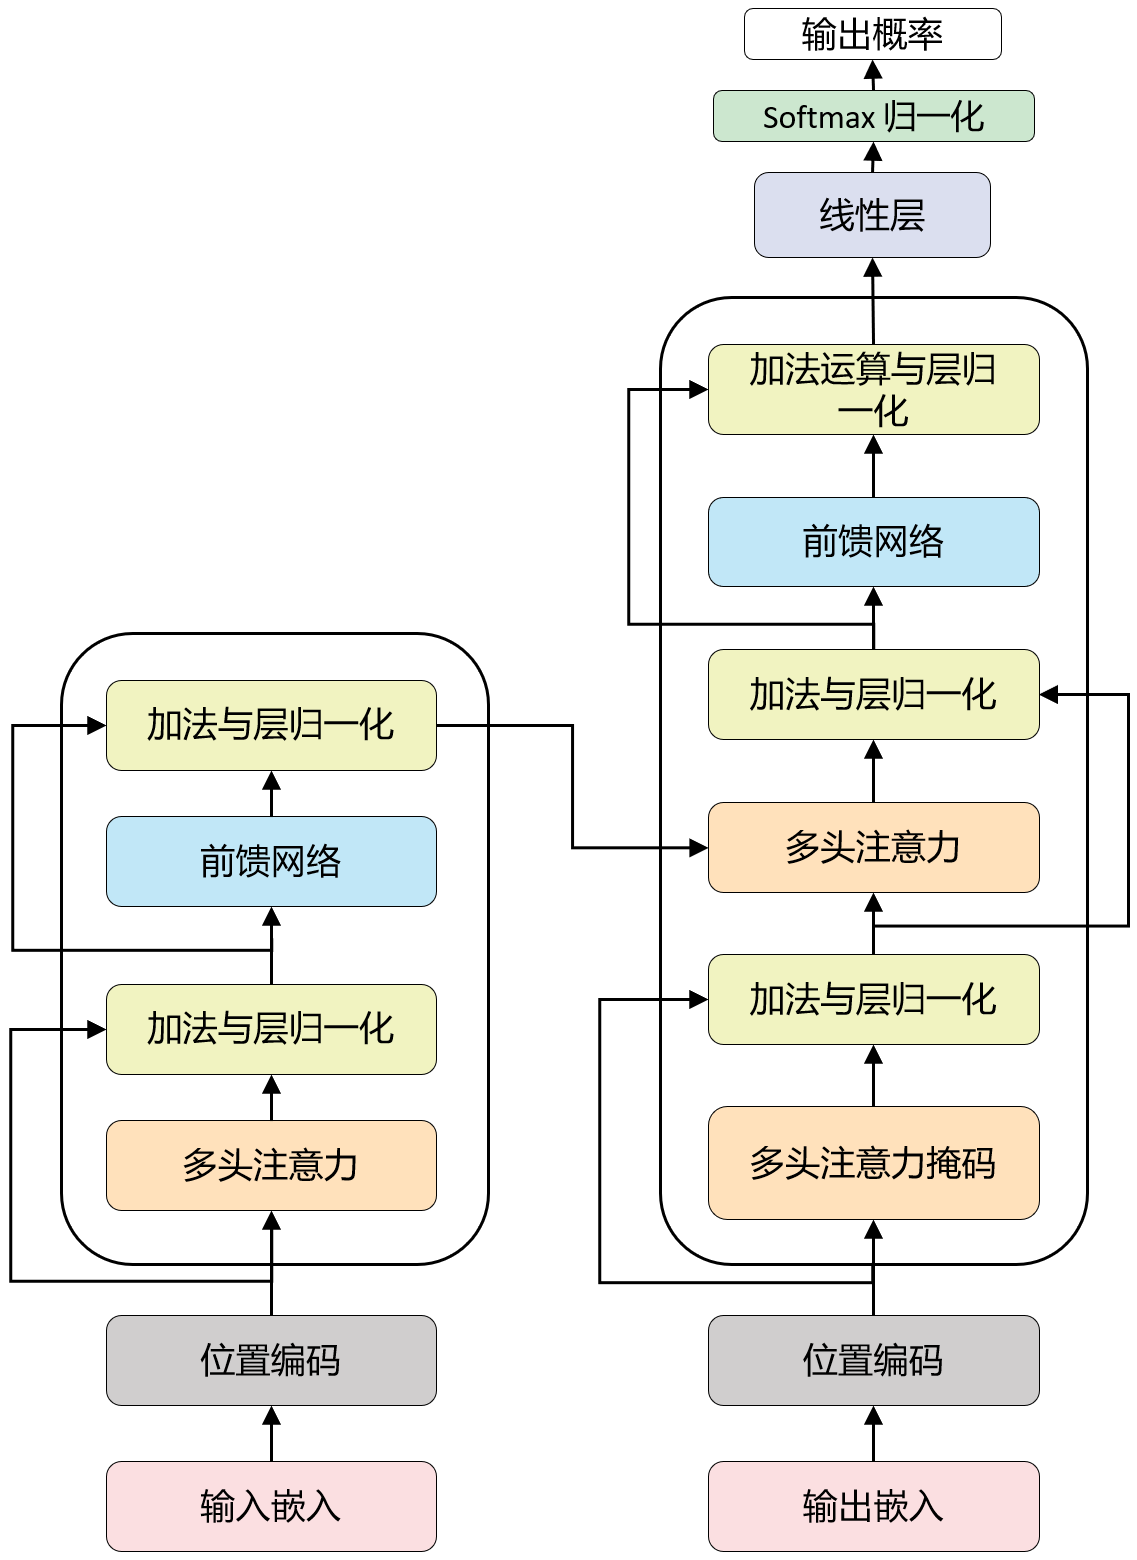
\includegraphics[width=0.82\textwidth]{Img/transformer_architecture_overview.png} \bicaption{Transformer 架构示意图}{Illustration of the Transformer architecture} \label{fig:chap2-transformer-architecture}
\end{figure} 如图~\ref{fig:chap2-transformer-architecture} 所示，Transformer 通常由输入嵌入、位置编码、多头自注意力、前馈网络以及残差归一化模块堆叠构成。其核心思想是在每一层中先通过自注意力完成全局依赖建模，再通过前馈网络对局部特征进行非线性变换，从而在保持并行计算能力的同时有效刻画长程上下文关系。这一结构优势也是后续 GPT、BERT、Qwen 等大语言模型能够持续扩展模型容量和上下文长度的重要基础。 在预训练阶段，Transformer 通常采用自回归语言建模或掩码语言建模两类目标学习通用表示。前者强调根据历史上下文预测下一个 token，适合生成式任务；后者通过恢复被遮蔽内容学习双向上下文表示，更适合理解类任务。本文引入 Qwen3 作为语义先验来源，正是建立在 Transformer 具备良好上下文建模和知识迁移能力这一基础之上。
\begin{figure}[htbp] \centering 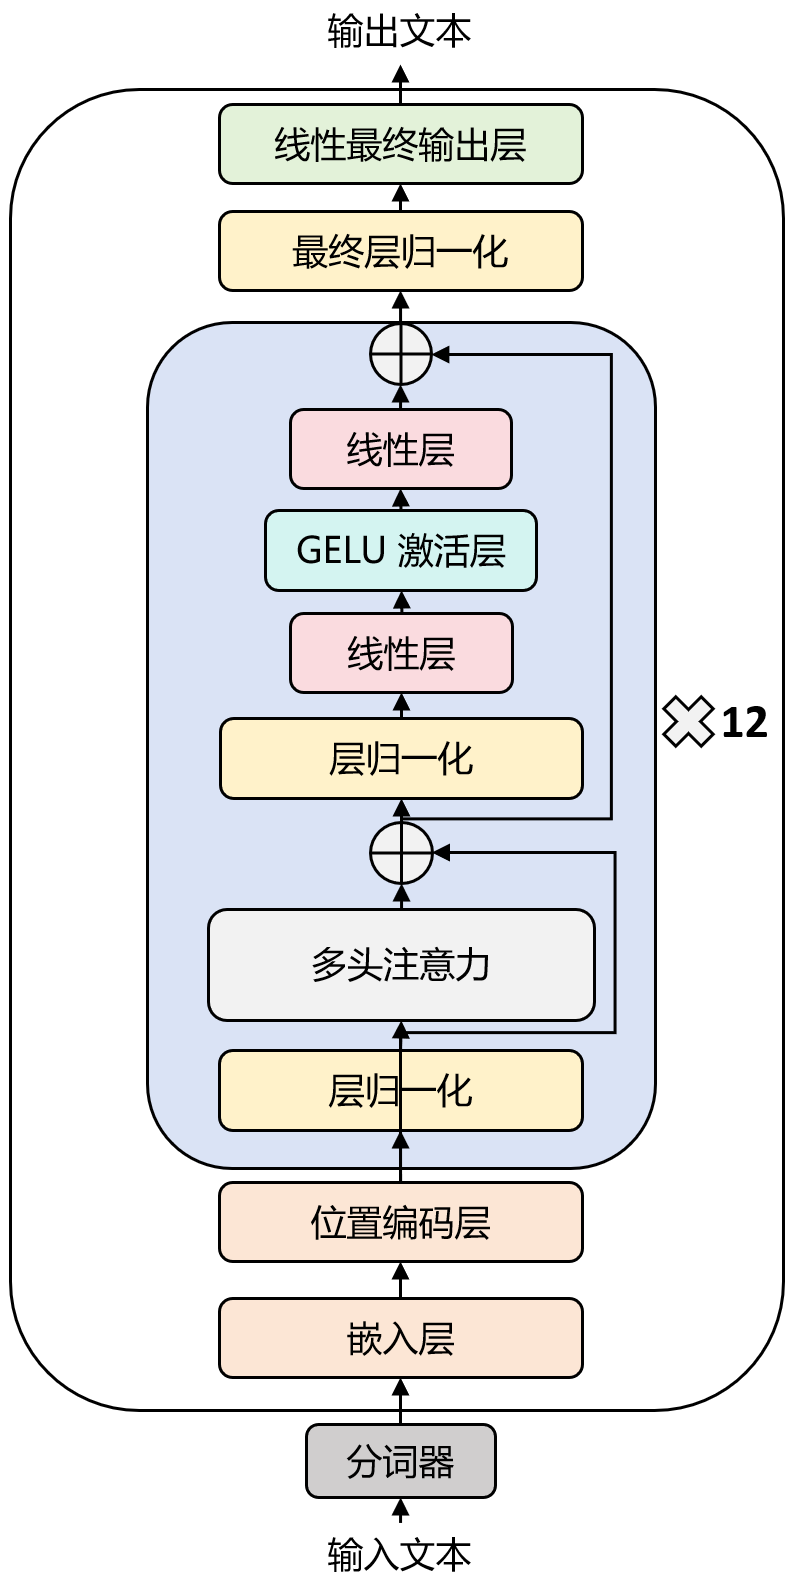
\includegraphics[width=0.54\textwidth]{Img/gpt2_architecture_overview.png} \bicaption{GPT-2 small 架构示意图}{Illustration of the GPT-2 small architecture} \label{fig:chap2-gpt2-architecture}
\end{figure} 如图~\ref{fig:chap2-gpt2-architecture} 所示，原始基线模型 T3Time 在语义分支中采用的是标准 GPT-2 small 作为外部语义编码器，其主体为解码器式 Transformer 堆叠结构，包含 12 层 Transformer block，隐藏维度为 768。在本文的实验设定中，GPT-2 主要承担原始语义骨干与对照基线的角色，用于刻画改进前统一预测骨架所依赖的语义表示来源。 随后，本文将其替换为 Qwen3-0.6B，以考察更先进的大语言模型表示能否继续提升统一预测骨架中的跨模态建模效果。相较于基线所使用的 GPT-2，Qwen3-0.6B 属于更新一代的轻量级稠密解码器模型，在参数规模仍然可控的前提下保留了更强的语义表示能力，因此更适合作为本文方法中的冻结语义先验来源\cite{yang2025qwen3}。 \begin{figure}[htbp] \centering 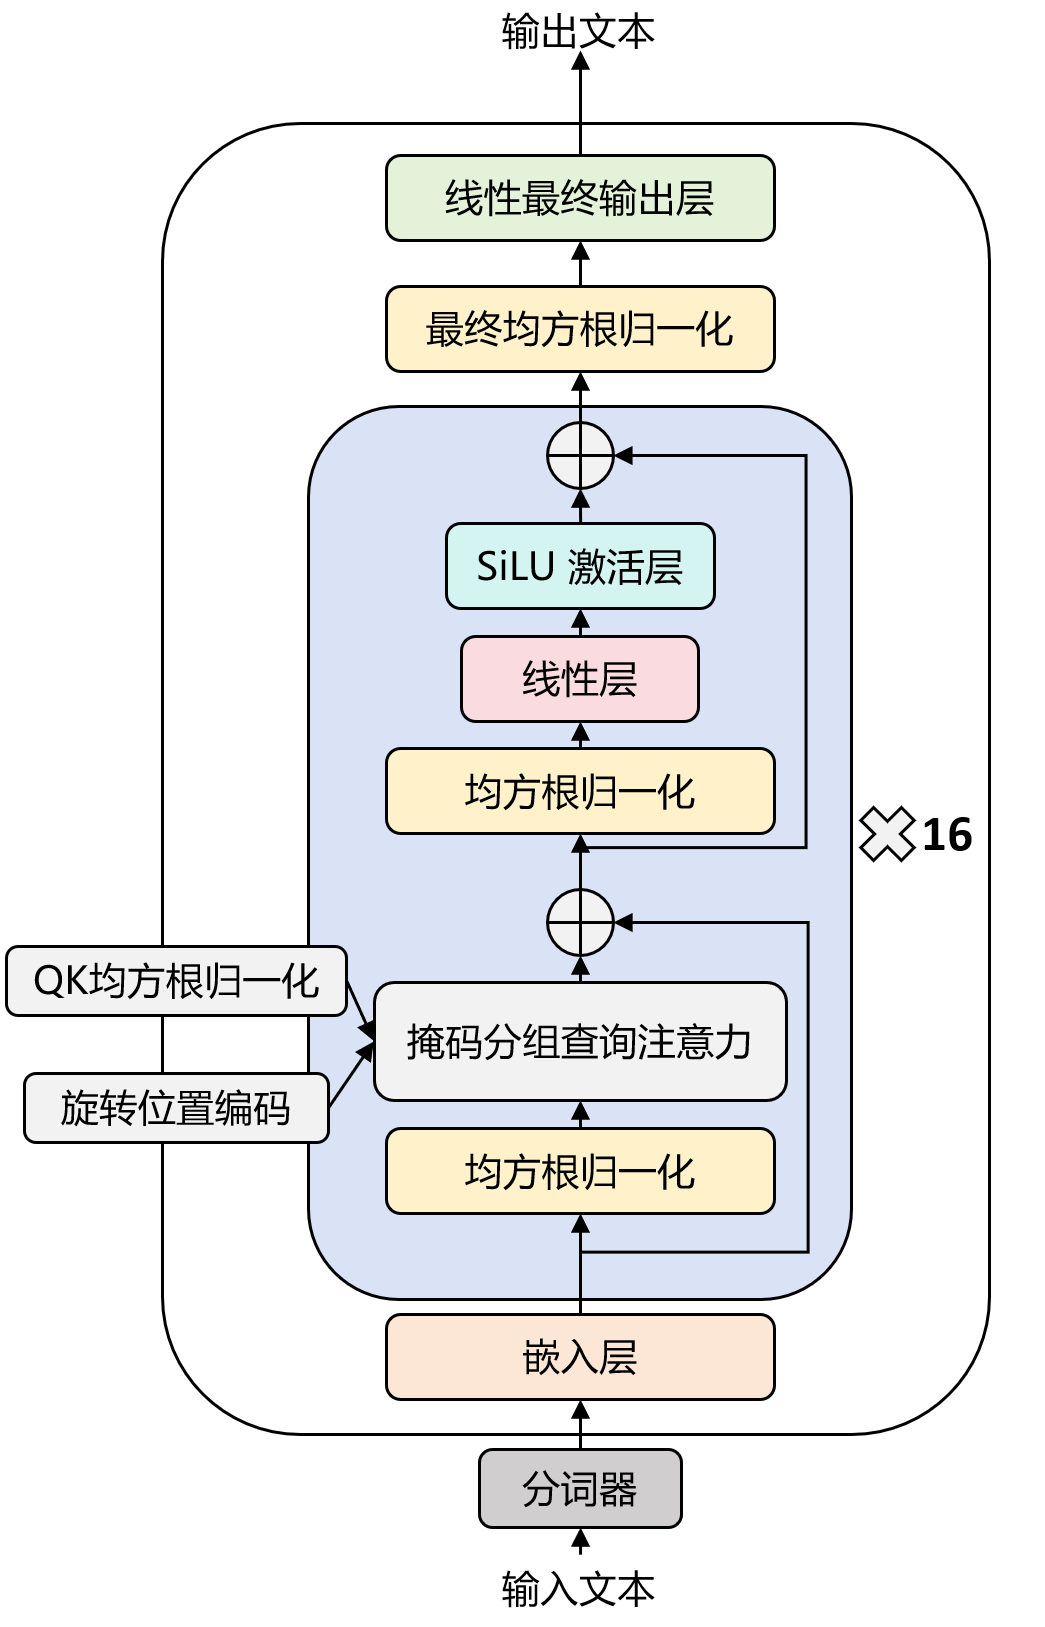
\includegraphics[width=0.58\textwidth]{Img/qwen_architecture_overview.png} \bicaption{Qwen3-0.6B 架构示意图}{Illustration of the Qwen3-0.6B architecture} \label{fig:chap2-qwen-architecture}
\end{figure} 如图~\ref{fig:chap2-qwen-architecture} 所示，Qwen3-0.6B 整体上延续了解码器式 Transformer 的主干结构，并在注意力、位置编码、归一化与前馈网络等关键位置采用更加适合长上下文建模与高效推理的结构设计。Qwen3-0.6B 采用自回归 Transformer 解码器架构，并结合 GQA、SwiGLU、RoPE、RMSNorm 和 QK-Norm 等设计，在推理效率、长上下文建模和训练稳定性之间取得了较好平衡。其中，GQA（Grouped Query Attention）通过让多个查询头共享较少数量的键值头，在尽量保持注意力表达能力的同时降低了推理阶段的键值缓存开销\cite{ainslie2023gqa}；SwiGLU 则在前馈网络中引入带门控的非线性激活结构，相较于传统激活函数通常具有更好的表达能力与训练稳定性\cite{shazeer2020glu}。RoPE（Rotary Positional Embedding）通过旋转位置编码将相对位置信息注入注意力计算过程，有助于增强模型对长上下文顺序关系的刻画能力\cite{su2021roformer}。RMSNorm 以均方根归一化替代标准 LayerNorm，在保持归一化效果的同时简化了计算过程\cite{zhang2019rmsnorm}；QK-Norm 则对 Query 和 Key 的表示尺度进行归一化约束，以缓解注意力分数波动过大的问题并提升训练稳定性\cite{henry2020qknorm}。这些设计共同构成了 Qwen3-0.6B 在效率、上下文建模能力与数值稳定性之间的平衡。 与基线模型所采用的 GPT-2 相比，Qwen3-0.6B 在模型设计与预训练能力上都更具先进性：前者注意力结构、位置编码与归一化方式相对基础，更强调通用文本生成能力；后者则在长上下文建模、数值稳定性与推理效率方面进行了系统优化。对于本文所研究的多元时间序列预测任务而言，我们并不直接依赖大语言模型生成预测值，而是将其作为冻结的外部语义编码器，用于提供变量级描述和任务背景的语义先验。在这一使用范式下，语义表示的区分性、稳健性和迁移能力比生成能力本身更为重要。相关电力系统综述也指出，将大语言模型引入复杂数值预测任务时，其潜在价值更多体现为知识迁移、语义建模与先验注入能力。因此，本文在保留统一预测骨架其余部分不变的前提下，将基线模型中的 GPT-2 语义骨干替换为 Qwen3-0.6B，并在第三章中通过对比实验验证这一替换带来的实际收益。 \section{时间序列频域分析理论} 时间序列不仅可以在时域上从值随时间变化的角度进行建模，也可以在频域上从不同频率成分的能量分布角度进行分析。频域方法通过将原始序列分解为一系列正弦/余弦基函数或其他频率基（如小波基），刻画序列中长期趋势、季节性周期以及高频波动等在频谱上的分布特征，有助于识别隐含的周期结构与多尺度模式。对于多元时间序列，通过在频域中分析不同变量在各频段上的能量与相干性，还可以更清晰地揭示跨通道的耦合关系。基于此，近年来大量长程时间序列预测工作开始引入傅里叶变换、小波变换以及频域神经网络等技术，将频域特征与时域深度模型相结合，以提升模型对长期周期性和复杂波动模式的刻画能力\cite{mallat1989wavelet}。相关中文教材也通常从联合时频分析角度解释频域方法在非平稳序列建模中的意义\cite{tang2016timefreqwavelet}。 \subsection{傅里叶变换及其局限性} 傅里叶变换是最经典的频域分析工具之一，其基本思想是将时间序列表示为一系列不同频率正弦和余弦函数的叠加。对于连续时间信号，可以将其理解为把时域信号投影到不同角频率的复指数基上，从而得到对应的频谱表示。对于长度为 T 的离散时间序列，常用的离散傅里叶变换（Discrete Fourier Transform, DFT）定义为 \begin{equation}
X(k) = \sum_{t=0}^{T-1} x_t\, e^{-j 2\pi kt / T}, \quad k = 0,1,\dots,T-1
\label{eq:chap2-12}
\end{equation}
其逆变换可以理解为将各个离散频率分量重新叠加，从而恢复原始时域序列。
在实际应用中，快速傅里叶变换（Fast Fourier Transform, FFT）可以在近似 T log T 量级的时间内高效计算 DFT，从而广泛应用于频谱估计、滤波和周期性分析等任务\cite{cooley1965algorithm}。通过观测幅度谱与功率谱，可识别序列中的主要频率成分及其能量分布，为后续的特征构造与模型设计提供重要先验。 尽管傅里叶变换在刻画全局周期结构方面具有坚实的理论基础和良好性能，但其在处理真实复杂时间序列时也存在若干局限性：第一，傅里叶基函数在整个时间轴上具有全局支撑，频谱表示缺乏时间局部性，难以刻画何时发生频率变化，即对非平稳或局部突变序列的时变特性表达能力有限；第二，傅里叶变换本质上假设信号在分析窗口内是平稳或近似平稳的，当序列统计特性随时间显著变化时，单一全局频谱难以反映局部结构差异；第三，标准傅里叶变换主要刻画幅度与相位信息，对于具有显著非线性、多尺度和间歇性特征的复杂信号，需要配合额外的时频局部化工具（如短时傅里叶变换、小波变换、小波包分解等）才能更全面地刻画其结构；第四，在深度学习框架下，直接在频域上进行操作时，如何在频谱稀疏性、相位信息利用与可微性之间取得平衡，也会对模型设计提出额外挑战。 因此，许多面向时间序列预测的频域方法往往并非仅依赖单一傅里叶变换，而是将其与其他方法相结合，既利用傅里叶频谱捕捉全局周期成分，也增强对局部突变与多尺度结构的刻画。本文在第四、五章中分别引入小波包分解与频域前馈网络，正是试图在傅里叶频域分析的基础上，进一步缓解上述局限性，为多元长程时间序列预测提供更具表达力的时频建模框架。
\subsection{小波包分解原理} 为克服傅里叶变换缺乏时间局部性的不足，小波及其变体提供了一种兼具时域与频域局部化能力的时频分析工具。中文教材中也从多分辨分析和工程信号处理角度对小波理论进行了较系统的阐述\cite{fan2008wavelet}。小波分析的基本思想是通过尺度函数提取信号的低频近似部分，通过小波函数提取局部高频细节，从而在不同尺度上同时刻画趋势与波动。对应地，尺度函数与小波函数满足经典的两尺度方程，其中低通分析滤波器负责保留信号中的缓慢变化趋势，高通分析滤波器负责提取边缘、突变及高频振荡等局部结构。

在连续形式下，信号可以表示为粗尺度近似项与多尺度细节项的叠加，这说明小波分析本质上是在多尺度框架下对信号进行趋势 + 细节的分层表示。对离散时间序列而言，离散小波变换可由正交滤波器组实现。对第 j 层输入序列进行分解时，其低频近似分量与高频细节分量分别可写为
\begin{equation}
a_k^{(j+1)}=\sum_{n} h[n-2k]x_n^{(j)}
\label{eq:chap2-17}
\end{equation}
\begin{equation}
d_k^{(j+1)}=\sum_{n} g[n-2k]x_n^{(j)}
\label{eq:chap2-18}
\end{equation}
式（\ref{eq:chap2-17}）和式（\ref{eq:chap2-18}）表明，离散小波分解可以理解为滤波 + 下采样的联合过程：低通支路保留信号的整体趋势与慢变化成分，高通支路则提取局部突变、边缘以及高频振荡信息。

然而，标准离散小波变换通常只继续分解低频近似部分，对高频细节的刻画仍然较为粗略。小波包分解（Wavelet Packet Decomposition, WPD）则进一步同时递归分解低频分量和高频分量，使子带数量随分解层数不断增加。其递归思想可以概括为：每一层都会对当前子带同时进行低通分解和高通分解，从而继续生成下一层的低频子带与高频子带。相比离散小波变换，小波包分解能更细致地描述中高频结构，因此更适合含有局部突变、多尺度波动和复杂非平稳特征的时间序列。

在本文中，多元时间序列的每个通道分别进行多层小波包分解，得到多尺度子带序列，并将其作为后续时频融合模块的输入。这样既保留了时间顺序信息，也显式强化了不同频段的能量分布表示，为第四章的局部波动增强建模提供基础。 \subsection{频域神经网络原理} 在频域视角下，时间序列可以通过离散傅里叶变换映射为一组复数频谱系数，从而将原本在时域中较难直接建模的长期周期性与全局模式转化为在频率轴上的能量分布与相位关系。传统深度模型多在时域上通过卷积或自注意力建模局部与长程依赖，而频域神经网络（尤其是频域多层感知机，Frequency-domain MLP, FreMLP）则尝试直接在频谱空间中进行特征变换与通道交互，利用频域的能量集中性与全局视角，构建更高效的时序建模机制。 一般而言，对长度为 L 的多元时间序列，若批大小为 B、通道数为 C，则沿时间维进行一维快速傅里叶变换（FFT）后可以得到复数频谱表示。对实序列而言，频谱长度通常对应半谱长度，也就是大约为原序列长度的一半再加一。频域神经网络的核心思想，是将该复数频谱拆分为实部与虚部，并在两部分上分别施加可学习的线性变换与非线性映射，从而在频域中显式建模不同变量之间、不同频率分量之间的联合关系。以本文采用的 FreMLP 形式为例，可对每个频率位置上的通道维进行复线性变换： \begin{equation}
\begin{aligned} \mathbf{O}_{\text{real}} &= \sigma\!\bigl(\Re(\mathbf{F})\,\mathbf{W}_r - \Im(\mathbf{F})\,\mathbf{W}_i + \mathbf{b}_r\bigr),\\ \mathbf{O}_{\text{imag}} &= \sigma\!\bigl(\Im(\mathbf{F})\,\mathbf{W}_r + \Re(\mathbf{F})\,\mathbf{W}_i + \mathbf{b}_i\bigr)
\end{aligned}
\label{eq:chap2-freq-complex-mlp}
\end{equation}
其中，两组权重矩阵负责分别建模实部与虚部之间的耦合关系，偏置项用于补充线性平移，激活函数则负责提供非线性表达能力。上述结构等价于对每个频率上的通道向量施加一个复值仿射变换，从而在频域中显式建模变量间的全局交互。随后可将更新后的实部与虚部重新组合为复数，并通过逆快速傅里叶变换（IFFT）回到时域，从而得到经频域 MLP 变换后的时域特征。由于 FFT 与 IFFT 均为可微操作，上述过程可以无缝嵌入端到端深度网络中进行联合训练。 为增强频域特征的稀疏性与鲁棒性，可进一步对复值输出施加 soft-shrink 等稀疏化算子，并结合门控机制在时域与频域之间进行自适应融合。本文第五章正是在这一思路下，将基础频域分支替换为基于 FreMLP 的频域前馈网络，以加强对全局周期结构和跨变量频谱关系的建模。 \section{门控注意力机制原理} \subsection{传统注意力机制的局限性} 自注意力机制（Scaled Dot-Product Attention, SDPA）是 Transformer 及大语言模型中的核心算子，其通过对查询（Query）、键（Key）和值（Value）之间的相似度进行加权求和来聚合上下文信息。对单个注意力头而言，标准缩放点积注意力会先计算 Query 与 Key 之间的相似度，再经过 Softmax 归一化得到注意力权重矩阵 A，并据此对 Value 进行加权汇聚。尽管该机制在捕捉长程依赖方面表现出色，但在大模型和长上下文场景下也暴露出若干局限性：

（1）\textbf{注意力分布过度集中的 attention sink 现象。} 实证研究表明，在预训练后的大模型中，某些特定位置（例如序列的首 token 或部分标点等非信息性 token）容易在多层多头注意力中获得异常高的注意力权重，即注意力汇聚或attention sink现象\cite{gu2024attentionsink}。这会导致大量上下文信息被无效地聚集到少数位置，降低注意力在有用上下文间的分辨能力，影响模型对细粒度模式的建模。

（2）\textbf{线性变换 + Softmax 的表达能力与稳定性瓶颈。} 标准注意力在查询与键的相似度矩阵之后仅通过 Softmax 引入单一的归一化非线性，缺乏更灵活的输入依赖变换空间。这既可能限制模型对复杂依赖关系的刻画，也会在大规模训练（特别是 BF16 等低精度训练）时让注意力输出与残差流中更容易出现massive activation（极大激活值），增加数值不稳定与梯度爆炸风险\cite{sun2024massive}。

（3）\textbf{难以自适应过滤无关上下文。} 传统注意力中，每个头在给定层内的 token 交互模式主要由查询与键的相似度矩阵和 Softmax 决定，虽然注意力权重本身依赖输入，但缺乏显式的、可解释的门控机制来对不同头、不同位置的输出进行幅度调节，从而在需要时主动压制与当前查询无关的上下文贡献。尤其在长上下文和多模态融合场景下，如何在不破坏有用依赖的前提下抑制冗余信息，是标准注意力难以直接解决的问题。

（4）\textbf{上下文长度扩展时的适配困难。} 在通过 RoPE 频率缩放、插值等技术扩展上下文长度时，原有注意力分布（尤其是 attention sink 模式）可能与新的位置编码不匹配，导致性能在长上下文下明显退化\cite{chen2023positioninterpolation,peng2023yarn}。缺乏显式控制信息流的手段，使得模型在零样本扩展到更长序列时难以及时调整注意力模式。

这些局限在大模型、长序列和多模态任务中尤为突出。引入门控机制后，可以在保留原有注意力结构优势的基础上，对注意力输出进行输入依赖、头依赖的显式调制，从而缓解注意力汇聚、数值不稳定和冗余信息干扰等问题。

\subsection{门控注意力的数学原理与优势}
门控注意力（Gated Attention）在标准注意力输出之上引入可学习的门控函数，通过对不同位置、不同注意力头的输出施加输入依赖的缩放因子，实现对信息流的精细控制。以对缩放点积注意力输出进行逐元素门控为例，可将标准注意力输出记为 H，并由当前层输入经过非线性映射生成门控系数 G，进而得到门控后的输出 \begin{equation}
\tilde{\mathbf{H}} = \mathbf{G} \odot \mathbf{H}
\label{eq:chap2-gated-attention-fused}
\end{equation}
其中，门控网络的输入通常取为当前层的查询表示或其线性变换；门控函数通常采用 Sigmoid 等能够将输出压缩到 0 到 1 区间的非线性函数；门控作用本质上表现为逐元素乘法。对于多头注意力，还可以在每个头上分别引入独立的门控，从而实现\textbf{头特定（head-specific）}的门控调制。 \begin{figure}[htbp] \centering 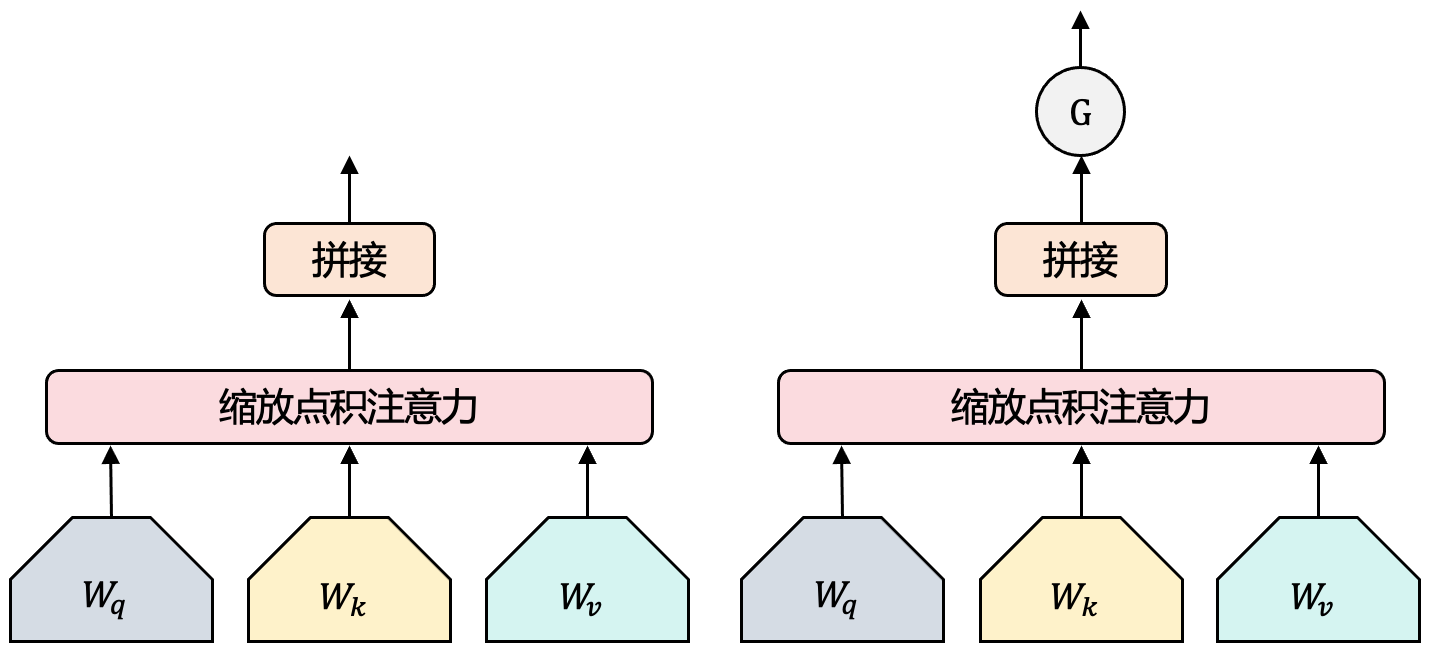
\includegraphics[width=0.72\textwidth]{Img/gated_attention_comparison.png} \bicaption{传统注意力与门控注意力对比示意图}{Comparison between conventional attention and gated attention} \label{fig:chap2-gated-attention-comparison}
\end{figure} 如图~\ref{fig:chap2-gated-attention-comparison} 所示，传统注意力通常直接将注意力权重作用于值向量并输出聚合结果，而门控注意力在此基础上进一步引入由输入驱动的门值，对不同位置或不同通道的信息流进行选择性缩放。该结构使模型不仅能够关注哪里，还能够进一步决定保留多少，因此在复杂上下文、多模态交互以及长序列建模场景下通常具有更强的特征筛选能力。门控注意力的优势主要体现在三个方面。第一，门控为注意力输出提供了额外的输入依赖非线性，有助于压制无关上下文。第二，门控可以减轻注意力过度集中和大激活值问题，提升训练稳定性。第三，该结构实现简单，易于与多模态融合和频域增强模块结合。本文在第三章利用门控思想完成多头跨模态输出的自适应融合，并在后续章节进一步扩展到时域和频域编码层中。 \section{数据集介绍} 为了系统评估本文提出的多元长程时间序列预测框架及其各个时频增强模块，本章选取了覆盖工业能耗、电力负荷、气象环境、公共卫生与金融市场等多种典型场景的公开基准数据集，并在统一的划分与预处理策略下进行对比实验。合理的数据集选择与规范的数据处理流程对于保证实验结论的客观性与可复现性至关重要，因此本节首先对所使用的数据集进行简要描述，随后介绍具体的数据划分方式与预处理步骤。
\subsection{数据集描述} 本文选取 ETTm1、ETTm2、ETTh1、ETTh2、Weather、ILI 和 Exchange 七个公开数据集进行评估，覆盖工业能耗、电力负荷、气象环境、公共卫生和金融市场等典型场景。例如，ETT 系列数据集由 Informer 工作构建并公开，用于检验模型对工业负荷与温度变化的长期预测能力；Weather 数据集来源于 Jena Climate 气象记录，能够反映复杂周期性与多变量相关性\cite{tensorflow2024jena}；Exchange 数据集采用 LSTNet 工作整理的多变量汇率序列，适合评估模型在金融时间序列上的非平稳建模能力\cite{lai2018lstnet}；ILI 数据集则基于美国 CDC FluView 发布的流感样病例周度监测数据构建，可用于分析公共卫生场景下的长期波动规律\cite{cdc2025fluview}。上述数据集在采样频率、变量维度和波动特性上差异明显，能够较全面地验证模型的泛化性能。 \begin{table*}[!htbp]
\centering
\scriptsize
\setlength{\tabcolsep}{4.5pt}
\renewcommand{\arraystretch}{0.9}
\bicaption{本文实验所用数据集统计信息}{Statistics of the datasets used in this thesis}
\label{tab:chap2-datasets}
\begin{tabular}{c|c|c|c|c|c}
\toprule
\textbf{数据集} & \textbf{维度} & \textbf{预测长度} & \textbf{数据集划分规模} & \textbf{采样频率} & \textbf{应用领域} \\
\midrule
ETTm1 & 7 & 96, 192, 336, 720 & 34465 / 11521 / 11521 & 15 分钟 & 电力 \\
\midrule
ETTm2 & 7 & 96, 192, 336, 720 & 34465 / 11521 / 11521 & 15 分钟 & 电力 \\
\midrule
ETTh1 & 7 & 96, 192, 336, 720 & 8545 / 2881 / 2881 & 1 小时 & 电力 \\
\midrule
ETTh2 & 7 & 96, 192, 336, 720 & 8545 / 2881 / 2881 & 1 小时 & 电力 \\
\midrule
Weather & 21 & 96, 192, 336, 720 & 36792 / 5271 / 10540 & 10 分钟 & 气象 \\
\midrule
Exchange & 8 & 96, 192, 336, 720 & 5120 / 665 / 1422 & 日度 & 汇率 \\
\midrule
ILI & 7 & 24, 36, 48, 60 & 617 / 74 / 170 & 周度 & 公共卫生 \\
\bottomrule
\end{tabular}
\end{table*} 表\ref{tab:chap2-datasets}对本文实验所使用数据集的维度、预测长度、数据划分规模、采样频率以及应用领域进行了汇总。其中，数据集划分规模按照训练集、验证集和测试集的顺序给出。除 ILI 数据集采用 24、36、48、60 作为预测长度外，其余数据集均采用 96、192、336、720 作为统一预测步长设置。
\subsection{数据预处理方法} 为保证不同模型之间的可比性，本文对所有数据集采用统一的数据预处理流程。首先，按照时间顺序划分训练集、验证集和测试集，避免未来信息泄漏。其次，在模型内部使用 RevIN 可逆归一化进行按变量归一化与反归一化，以减小量纲差异和分布漂移带来的影响。再次，采用滑动窗口方式构造输入输出样本对\cite{kim2022revin}。对于 ETTm1、ETTm2、ETTh1、ETTh2、Weather 和 Exchange 六个数据集，统一设置历史窗口长度为 96，预测步长为 96、192、336、720，以评估模型在标准长程预测场景下的表现。 ILI 数据集的时间粒度为周度，整体样本规模也显著小于其余数据集。若仍采用与高频数据集相同的超长预测设置，会导致有效训练样本数量不足，并明显加剧长程外推难度。因此，本文对 ILI 数据集采用单独的窗口配置：输入历史长度设为 36，预测步长设为 24、36、48、60。其中，这四组预测长度分别对应较短、中等和较长的周度预测范围，更符合 ILI 数据集的采样频率与任务特点，也与现有公开时间序列预测工作中的常见设置保持一致。 对于带有时间戳的数据集，本文进一步提取小时、星期、月份等周期性时间特征作为辅助输入，以帮助模型建模潜在的时间周期规律。除 ILI 在输入窗口和预测步长上采用专门设置外，其余数据集均遵循统一的标准长程预测预处理流程，从而保证后续实验结果具有良好的可复现性与横向可比性。
